\begin{surferPage}[216 Singularidades]{Superficies con muchas singularidades}
    El valor exacto de singularidades de una superficie de grado $7$, $\mu(7)$, no es conocido.
    Pero se sabe que: $99\le \mu(7) \le 104$. Naturalmente, se tiene menos idea en superficies de grado superior.
    
    En $2005$, Sonja Breske, Oliver Labs y Duco van Straten, mediante una adaptación de 
    una construcción de Chmutov $(1992)$, consiguieron establecer que el número máximo de puntos singulares
    obtenido hasta el momento se puede alcanzar también por superficies reales con singularidades reales.
    
    Este resultado es la cota inferior de la siguiente desigualdad (la cota superior se debe a Miyaoka):
    \[0,41\bar{6}d^3 \lessapprox \mu(d) \lessapprox 0.44\bar{4} d^3.\]
     En las imágenes podemos ver la simetría de la construcción, y su relación
     con el número máximo de áreas negras en el gráfico de rectas:
    \begin{center}
      \begin{tabular}{c@{\qquad}c}
        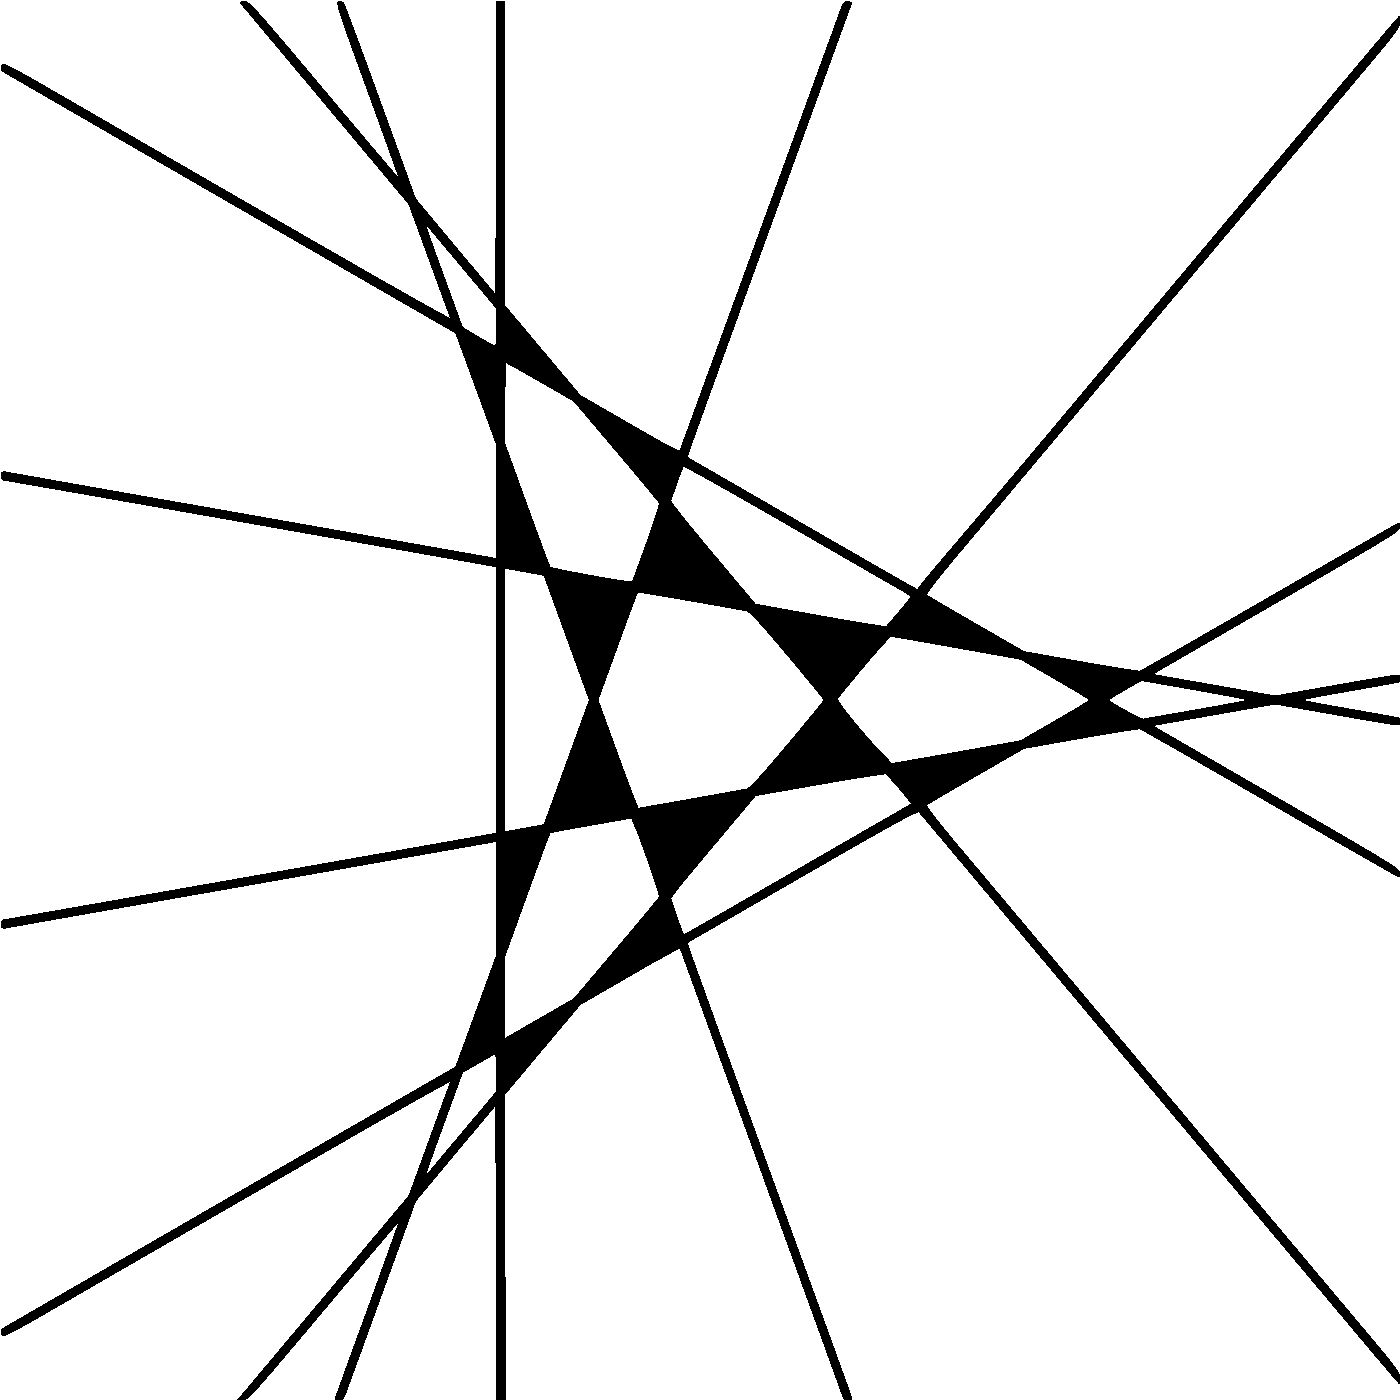
\includegraphics[height=1.5cm]{../../common/images/vielesing.pdf}
        &
        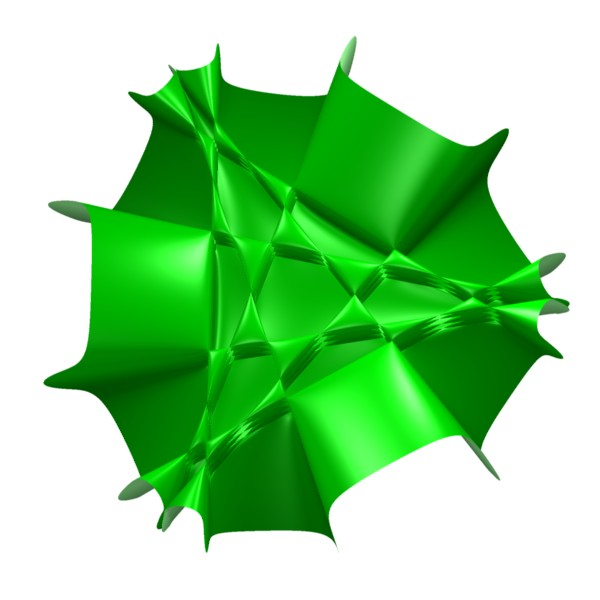
\includegraphics[height=1.5cm]{../../common/images/p9surface_von_oben}
      \end{tabular}
    \end{center}
\end{surferPage}
